The bunch crossing rate at LHC is 40~MHz for a bunch spacing of 25~ns (about 7
meters). Each event recorded by ATLAS requires $\approx 1.4$~MB of disk space,
with approximately 20 to 50 collisions per bunch crossing, the storage space
required to record all the events in a second would be $\approx 60$~TB. This is
not feasible thus only the most interesting events are selected and stored on
disk. The \emph{trigger system} decides whether to keep or not a collision event
for later studies, it consists of a hardware based \gls{l1} trigger and a
software based \gls{hlt}.

The L1 trigger determines \gls{rois} in the detector using custom hardware and
coarse information from the calorimeter and the muon system. The L1 trigger is
capable of reducing the event rate to 100~kHz with a decision time for a L1
accept of 2.5~$\mu$s. The RoIs from the L1 trigger are sent to the HLT where
different algorithms are run using the full detector information and reducing
the L1 output rate to 1~kHz with a processing time of about
200~ms~\cite{trigger}. %A schematic overview of the ATLAS trigger and data
%acquisition system is shown in Figure~\ref{fig:trigger_system}.

In the 2015 monojet analysis presented in this thesis, the HLT\_xe70 trigger is
used, it receives an L1 accept that selects events with a missing energy (see
\cref{sec:miss-transv-energy}) greater than 50~GeV, no muons are used in the
reconstruction of the missing energy at the trigger level. The events that
survive L1 are then passed to the \gls{hlt} level, where events with a missing
energy greater than 70~GeV are selected.

In the 2016 analysis a combination of four different triggers is used, they all
pass the level one trigger selection if the event have a missing energy of more
than 50~GeV, again no muon information is used in the missing energy
reconstruction at this level. For the \gls{hlt} the missing energy threshold is
increased in steps of 10~GeV from 80~GeV up to 110~GeV for the four different
triggers. The information on the missing energy takes advantage of the \gls{mht}
algorithm or the \gls{lcw} calibration scheme depending on the trigger used. In
the \gls{mht} algorithm the missing energy is calculated as the negative vector
sum of the transverse momentum
($- \sum \pt^\mathrm{\, jets} \equiv - H_\mathrm{\, T}$) of all the jets
reconstructed with the $\antikt$ jet finding algorithm (see \cref{sec:anti-k_t})
from topoclusters (see \cref{sec:topocluster})~\cite{MHTAlgorithm}. The
\gls{lcw} calibration scheme uses the shape of the cluster and the energy
density to classify the topocluster energy deposits as electromagnetic or
hadronic improving the resolution of the missing energy
trigger~\cite{LCWCalibration}. \cref{tab:trigger_periods} summarizes the
different trigger combination for the 2016 dataset used in the analysis. The
increase with time of the average number of interactions per bunch crossing
($\langle \mu \rangle$) forced the use of a higher missing energy threshold in
the trigger. \cref{fig:trigger_efficiency} shows the trigger efficiency for the
four different data taking periods in the 2016 analysis as a function of the
missing energy estimated using $\wmunuplusjets$ events. It can be seen that the
trigger is fully efficient from approximately 200~GeV.
% receive an L1 accept for events with more than 50~GeV of missing energy, with no
% muon information for the missing energy reconstruction at this level.
% HLT\_xe80\_tc\_lcw\_L1XE50, HLT\_xe90\_mht\_L1XE50,
% HLT\_xe100\_mht\_L1XE50 and HLT\_xe110\_mht\_L1XE50. The
% HLT\_xe80\_tc\_lcw\_L1XE50 at L1 level selects events with a missing energy of
% more than 50~GeV while at the \gls{hlt} level it uses the \gls{lcw} to calibrate
% the missing energy whose information is taken from the energy deposited in the
% topocluster (tc) (see \cref{sec:topocluster}). The \gls{lcw} uses the
\begin{table}[!hb]
  \centering
  \begin{tabular}{lcc}
    \toprule
    \multicolumn{3}{c}{Trigger Used In The 2016 Data Taking} \\
    \midrule \midrule
    Run Range & Trigger & $\langle \mu \rangle$ \\
    \midrule
    296939-302393 & HLT\_xe90\_mht\_L1XE50 or HLT\_xe80\_tc\_lcw\_L1XE50 & 33.1 \\
    302737-302872 & HLT\_xe90\_mht\_L1XE50 & 34 \\
    302919-304008 & HLT\_xe100\_mht\_L1XE50 or HLT\_xe110\_mht\_L1XE50 & 35.4 \\
    304128-310216 & HLT\_xe110\_mht\_L1XE50 & 51.1 \\
    \bottomrule
  \end{tabular}
  \caption{The table reports the trigger used in the 2016 data taking. The
    average number of interactions per bunch crossing, $\langle \mu \rangle$, is
  also reported. The constant increasing of $\langle \mu \rangle$ justifies the
  choice of higher $\met$ thresholds for the trigger.}
  \label{tab:trigger_periods}
\end{table}
\begin{figure}[!ht]
  \centering
    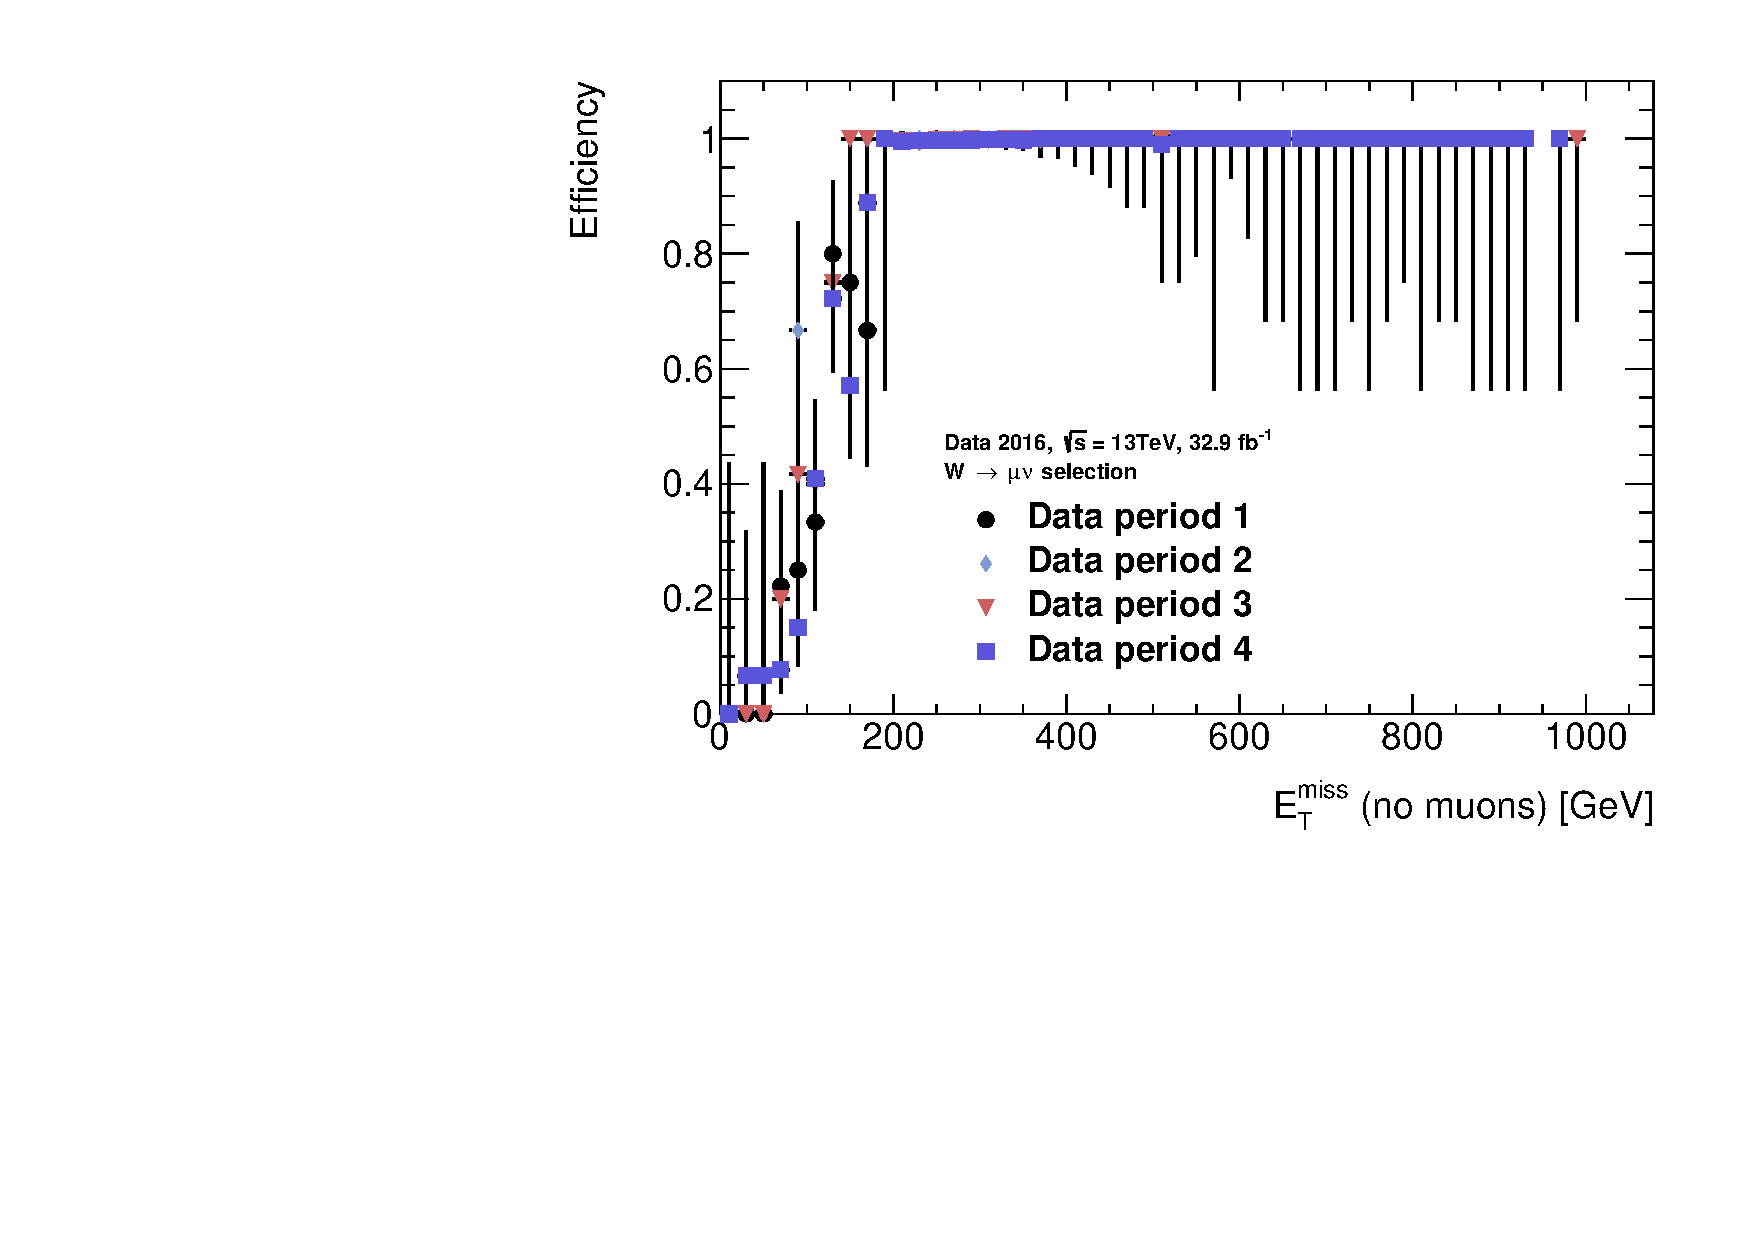
\includegraphics[width=\linewidth]{trigger_efficiency}
    \caption{Trigger efficiency curve as a function of the missing energy for
      the 2016 dataset of 32.9~$\ifb$ estimated in $\wmunuplusjets$ events. The
      trigger is fully efficient from approximately 200~GeV.}
    \label{fig:trigger_efficiency}
\end{figure}
% \begin{figure}[!h]
%   \centering
%     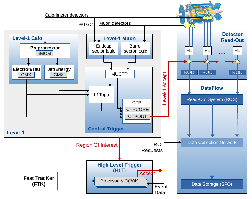
\includegraphics[width=.7\linewidth]{trigger_system}
%     \caption{Schematic view of the ATLAS trigger and data acquisition system.}
%     \label{fig:trigger_system}
% \end{figure}
%%% Local Variables:
%%% mode: latex
%%% TeX-master: "../search_for_DM_LED_with_ATLAS"
%%% End:
